\documentclass[conference]{IEEEtran}
\IEEEoverridecommandlockouts
\usepackage{cite}
\usepackage{amsmath,amssymb,amsfonts}
\usepackage{algorithmic}
\usepackage{graphicx}
\usepackage{textcomp}
\usepackage{xcolor}
\def\BibTeX{{\rm B\kern-.05em{\sc i\kern-.025em b}\kern-.08em
    T\kern-.1667em\lower.7ex\hbox{E}\kern-.125emX}}
\begin{document}

\title{POME: [Project Full Title]\\
{\footnotesize \textsuperscript{*}Project Paper - [Course/Conference Name]}
}

\author{\IEEEauthorblockN{Team Member 1}
\IEEEauthorblockA{\textit{Department/Major} \\
\textit{University/Organization}\\
City, Country \\
email@example.com}
\and
\IEEEauthorblockN{Team Member 2}
\IEEEauthorblockA{\textit{Department/Major} \\
\textit{University/Organization}\\
City, Country \\
email@example.com}
\and
\IEEEauthorblockN{Team Member 3}
\IEEEauthorblockA{\textit{Department/Major} \\
\textit{University/Organization}\\
City, Country \\
email@example.com}
}

\maketitle

\begin{abstract}
% Abstract content - included via \input in main.tex's abstract environment
One of the questions which software product teams are likely to face in this era of high technological change is how and what to do with such a multitude of various kinds of features prior to being able to allocate resources based on prospective information regarding the demand in a product design process.

The focal point of the proposed study is Notion, which is a tremendously popular SaaS (Software as a Service) productive platform, as data analytics models owned by the proprietors cannot be shared publicly, and, instead, the data on search interest in Google Trends, app store review corpora, and user-feedback patterns can be publicly available to generate a specific demand signal of a particular feature of a product.

The proposed forecasting system would employ an ensemble technique of sampling that incorporates different methods of analysis, which include Exponential Smoothing, ARIMA and linear regression models. The different approaches would thus enable the different concerned parties to have a picture of the larger picture.

As the empirical evidence indicates, it is evident that it is possible to recognise the recognisable trends in the analysed attributes, including AI-driven features, template features, and automation processes. The trends in the development of AI-related factors include long-term growth curves, templates possess stable bases of demand, with predictable seasonal variation, and automation capability, and the automation features have intermediate growth rates with regard to the workflow optimization trends in the industry.

The core worth on the work is the clarification that one can only identify meaningful demand forecasting through pure utilisation of publicly accessible data in determining the prioritisation of software features. The explanation is that companies with limited analytical ability can only reduce the extent to which development resources are misplaced and also improve the alignment between product roadmap and user demands.

\textbf{Index Terms}---SaaS product management, demand forecasting, time series analysis, feature prioritisation, Google Trends, sentiment analysis, ARIMA, exponential smoothing.

\end{abstract}

\begin{IEEEkeywords}
[Add relevant keywords for your project, e.g., machine learning, data analysis, software engineering, etc.]
\end{IEEEkeywords}

% Include section files
\section{Introduction}

Software-as-a-Service (SaaS) products are now crucial for personal productivity, team collaboration, and digital workflows. Among the many tools available, Notion stands out as one of the most flexible platforms. It offers modular databases, templates, workspace organization, and recently, AI-powered features. As the platform grows, product teams face the challenge of deciding which features to design or improve at any time. Relying solely on developer intuition or limited feedback is not enough in today's competitive market. Instead, using data-driven forecasting can provide clear insights into emerging user needs.

Demand forecasting in SaaS means predicting user interest in specific features by examining trends in search behavior, usage patterns, review sentiments, and external events. This is different from forecasting in traditional industries because the demand for SaaS features is nonlinear; it is often swayed by competitor launches, viral content, or sudden shifts in work habits. Recognizing upcoming demand early allows product designers to make better choices regarding UI/UX, workflows, design complexity, and engineering investment.

This study looks at how to adapt forecasting methods to SaaS environments using publicly available datasets. We center on Notion as a case study because of its large user base, active online communities, and open feature discussions. By modeling demand trends for features like Notion AI, templates, and automation workflows, the study shows how forecasting helps guide design decisions. The goal is to demonstrate that forecasting is not just a technical tool; it serves as a strategic foundation for creating products that stay relevant, intuitive, and effective.

\subsection{Background and Motivation}
SaaS productivity platforms work in a quickly changing environment where user expectations shift often, and new workflow patterns arise regularly. In this setting, creating the right features at the right time is essential for product success. Since internal analytics from SaaS companies are not publicly available, this study develops a forecasting method based on publicly accessible proxy datasets like Google Trends data, app review datasets, and user feedback trends specific to features.

\subsection{Problem Statement}
Product teams in SaaS companies must decide which features to prioritize, improve, or redesign without always having access to comprehensive internal analytics. Traditional approaches relying on developer intuition or limited user feedback are insufficient in today's competitive and rapidly evolving market. There is a need for a data-driven approach that can predict feature demand and inform design decisions effectively.

\subsection{Research Objectives}
The objectives of this research are:
\begin{itemize}
\item To understand how interest in different Notion features changes over time by studying publicly available data like Google Trends and user reviews
\item To use forecasting methods such as Exponential Smoothing, ARIMA, and Regression to predict which Notion features are likely to become more or less popular in the future
\item To explore how these demand predictions can guide real product decisions, such as which features should be improved, prioritized, or redesigned
\item To build a practical and easy-to-follow framework that software teams can use to connect demand insights with better UI/UX design and release planning
\end{itemize}

\subsection{Scope and Significance}
This study aims to create a simple and replicable forecasting framework that software companies can use, even without access to large internal datasets. The overall goal is to demonstrate that effective demand forecasting not only helps companies create better features but also ensures that product design keeps up with user needs, which can reduce churn and improve product adoption. The research focuses specifically on Notion as a case study but provides a methodology applicable to other SaaS platforms.

\subsection{Organization of the Paper}
The remainder of this paper is organized as follows: Section II reviews related work in demand forecasting and feature prioritization. Section III presents the system design and architecture. Section IV describes the methodology in detail. Section V discusses the implementation approach. Section VI presents testing procedures and evaluation metrics. Section VII provides results and findings. Section VIII discusses the implications and limitations. Section IX outlines team contributions. Section X suggests future work, and Section XI concludes the paper.

\section{Related Work}

The section provides the review of the literature on the subject of the suggested framework, analysing the previous studies in the field of demand forecasting, feature prioritisation, time series analysis, and sentiment analysis. The review reveals the gaps in existing solutions, which this study fills.

\subsection{Software Feature Demand Forecasting}
The conventional research in demand forecasting started in the setting of physical products---consumer goods, electronics and retail inventory. Box and Jenkins models of ARIMA are still in use today as they are robust and can be interpreted. Nevertheless, software capabilities have different peculiarities that distinguish the product of software, in comparison with tangible goods. The demand for features is not subjected to any predictable seasonal pattern and can fluctuate fast, in response to the announcements of viral content, rivalry, or changes in user behaviour. It has been established that the trends in internet search are significantly correlated with real-life patterns of interest. Search data has been used to forecast phenomena as diverse as financial market trends, and epidemiological trends. This theoretical reasoning has been supported by the fact that search behaviour as an indicator of true user interest, is the premise upon which publicly available search data are used as a proxy of demand. It is an understanding that motivated the use of Google Trends data as one of the main demand signals in this model.

\subsection{Prioritisation of Features on SaaS Products}
The product management practitioners use many prioritisation models such as RICE scoring, Kano models and value-versus-effort matrices. Although these frameworks offer formal systems of decision making, they need considerable subjectiveness. Practitioners need to approximate the effect, gauge user worth, and prioritise the features according to in-house deliberations. These methods are sufficient in the case of simple products, but they scale poorly and are prone to numerous types of cognitive biases. There are other organisations that have implemented analytics-based prioritisation approaches that use internal usage data to make roadmap decisions. Nonetheless, this internal data is owned and not available to any external researchers, so it is not possible to study, replicate, and generalise results across products. This study solves this weakness by showing that publicly accessible data has enough signal strength to be used to make decisions on the prioritisation of features.

\subsection{Time Series and Machine Learning}
Methods of forecasting are across a continuum between traditional statistical processes and modern machine learning techniques. Traditional methods such as Exponential Smoothing and ARIMA models are easily interpretable, have a solid theoretical basis, and do not require extensive data. Neural networks, gradient boosting, random forests, the various machine learning methods, are able to learn complex, non-linear patterns but usually need more and less interpretable data. Comparative experiments show that the simpler models often perform competitively with respect to more complex alternatives especially using small datasets. To the current use case, i.e. predicting interest in particular software features with the help of public data, an ensemble of classical methods can offer the right level of accuracy and interpretability. Current research on scalable forecasting has shown that hybrid systems that incorporate statistical rigour with practical implementation strategies are showing excellent results.

\subsection{Sentiment Analysis and User Feedback}
The feedback provided by users is one of the most useful sources of information about user sentiment, as it is taken in the form of reviews in the app shops and discussions in social media. NLP methods allow studying extensive review collections in order to identify feature mentions, pain points, and satisfaction patterns. Sentiment analysis gives extra information about what is discussed by the users in addition to their emotional inclination towards certain features. Other literature in this field has concentrated more on the existing user perceptions about existing features. The study is unique in that it tries to forecast future demand and not just quantify the current sentiment. Nevertheless, temporal patterns in sentiment have the potential to mean demand trends, which is why sentiment analysis should be implemented into a forecasting model.

\subsection{Research Gap and Contribution}
The research void that the study will fill is that there are no unified frameworks relating to the design of SaaS products in terms of forecasting, prioritisation, and sentiment analysis. Traditionally forecasting research has been concerned with the physical products. The systems of priorities are still qualitative. The work of sentiment analysis is mainly retrospective instead of being predictive. This paper forms a framework that incorporates these lines of research. Using a combination of forecasting methods, testing on empirical trends in features, and only using publicly available data, this study shows a practical method that can be used by a product team that does not have a large analytical infrastructure. It is methodological but not algorithmic in nature of contribution---larger teams are made available to small teams of data-driven decision-making capabilities that would otherwise require large analytical resources.

% System Design and Architecture Section
% Describe the overall system design and architecture

\section{System Design}

\subsection{System Architecture}
The system follows a modular pipeline architecture consisting of four main stages that transform raw public data into actionable design insights. The architecture is designed to be scalable, reproducible, and adaptable to various SaaS platforms beyond Notion.

The system operates as a sequential pipeline where each stage feeds into the next:
\begin{enumerate}
\item \textbf{Data Collection Layer}: Aggregates publicly available demand signals from multiple sources including Google Trends API, Kaggle review datasets, and app metadata repositories
\item \textbf{Data Preprocessing Layer}: Cleans, normalizes, and organizes raw data into feature-specific time series suitable for forecasting models
\item \textbf{Forecasting Engine}: Applies multiple time-series forecasting techniques (Exponential Smoothing, ARIMA, Linear Regression) to generate demand predictions
\item \textbf{Design Decision Framework}: Translates forecast outputs into concrete product design recommendations including feature prioritization, UI/UX optimization strategies, and resource allocation guidance
\end{enumerate}

The architecture emphasizes modularity, allowing each component to be updated or replaced independently. Data flows unidirectionally from collection through decision-making, with feedback loops enabling continuous refinement of forecast models based on validation results.

\subsection{Component Design}

\subsubsection{Data Collection Module}
This module serves as the entry point for all external data sources. It implements:
\begin{itemize}
\item \textbf{Google Trends Scraper}: Collects monthly search interest data for specific Notion features (e.g., "Notion AI", "Notion templates", "Notion automation")
\item \textbf{Review Dataset Parser}: Processes Kaggle datasets containing user reviews, ratings, and timestamps from app stores
\item \textbf{Metadata Aggregator}: Gathers app installation counts, version releases, and rating distributions
\end{itemize}

All collected data is timestamped and stored in a standardized format to ensure consistency across different data sources. The module handles API rate limiting, data validation, and error recovery to maintain data quality.

\subsubsection{Data Preprocessing Module}
This component transforms raw data into analysis-ready formats:
\begin{itemize}
\item \textbf{Data Cleaning}: Removes duplicates, handles missing values, and filters outliers
\item \textbf{Feature Extraction}: Uses Natural Language Processing (NLP) techniques to extract feature mentions from user reviews and feedback
\item \textbf{Sentiment Analysis}: Applies sentiment scoring to reviews to gauge user satisfaction with specific features
\item \textbf{Time Series Construction}: Organizes data into monthly time series for each Notion feature, including search interest, sentiment scores, and mention frequencies
\item \textbf{Normalization}: Scales data across different metrics to enable cross-feature comparison
\end{itemize}

\subsubsection{Forecasting Engine}
The core analytical component that generates demand predictions using three complementary approaches:
\begin{itemize}
\item \textbf{Exponential Smoothing Model}: Captures short-term demand shifts and recent trends, particularly useful for identifying sudden interest spikes
\item \textbf{ARIMA (AutoRegressive Integrated Moving Average)}: Models long-term patterns, seasonality, and cyclical behaviors in feature demand
\item \textbf{Linear Regression Model}: Analyzes the impact of external factors (e.g., competitor releases, viral events) on demand trajectories
\end{itemize}

Each model produces independent forecasts that are then ensemble-weighted based on historical accuracy. The engine outputs confidence intervals alongside point predictions to support risk-aware decision-making.

\subsubsection{Design Decision Framework}
This module interprets forecast outputs and generates actionable design recommendations:
\begin{itemize}
\item \textbf{Feature Prioritization Engine}: Ranks features based on predicted demand growth, current sentiment, and strategic importance
\item \textbf{UI/UX Optimization Advisor}: Recommends interface changes for high-demand features (e.g., improved discoverability, simplified workflows)
\item \textbf{Resource Allocation Planner}: Suggests engineering effort distribution based on demand forecasts and implementation complexity
\item \textbf{Release Planning Tool}: Identifies optimal timing for feature launches or updates based on predicted demand peaks
\end{itemize}

The framework uses rule-based logic combined with threshold-based triggers to translate quantitative forecasts into qualitative design actions.

\subsubsection{User Interface Module}
The User Interface (UI) module provides an interactive view of forecasts and recommendations for product designers and stakeholders. It implements:
\begin{itemize}
\item \textbf{Dashboard Views}: Aggregated metrics and trend visualizations to surface high-level demand movements.
\item \textbf{Feature Drill-downs}: Per-feature time series, sentiment overlays, and model comparison widgets to inspect drivers of demand.
\item \textbf{Actionable Recommendations}: UI elements that present prioritized feature suggestions, estimated effort, and suggested release windows derived from the Design Decision Framework.
\item \textbf{Export and Reporting}: CSV/JSON export options and printable reports to support offline review and decision-making.
\end{itemize}

The UI module is intentionally decoupled from the forecasting engine so that improvements to visualization or interaction design do not affect core analytics logic.

\subsection{Technology Stack}

\subsubsection{Programming Languages}
\begin{itemize}
\item \textbf{Python 3.x}: Primary language for data processing, statistical analysis, and forecasting model implementation due to its rich ecosystem of data science libraries
\item \textbf{SQL}: For structured data storage and querying of time-series datasets
\end{itemize}

\subsubsection{Frameworks and Libraries}
\begin{itemize}
\item \textbf{pandas}: Data manipulation and time-series handling
\item \textbf{NumPy}: Numerical computations and array operations
\item \textbf{statsmodels}: Implementation of ARIMA and Exponential Smoothing models
\item \textbf{scikit-learn}: Linear regression, data preprocessing, and model evaluation metrics
\item \textbf{NLTK / spaCy}: Natural Language Processing for feature extraction from reviews
\item \textbf{TextBlob / VADER}: Sentiment analysis of user feedback
\item \textbf{matplotlib / seaborn}: Data visualization and forecast plotting
\item \textbf{pytrends}: Google Trends API interface for search interest data collection
\end{itemize}

\subsubsection{Data Sources and Storage}
\begin{itemize}
\item \textbf{Google Trends API}: Search interest time-series data
\item \textbf{Kaggle Datasets}: App review collections and user feedback data
\item \textbf{CSV/JSON Files}: Lightweight storage for collected and preprocessed data
\item \textbf{SQLite / PostgreSQL}: Relational database for structured time-series storage (optional for larger deployments)
\end{itemize}

\subsubsection{Development and Collaboration Tools}
\begin{itemize}
\item \textbf{Jupyter Notebooks}: Interactive development, exploratory data analysis, and model prototyping
\item \textbf{Git / GitHub}: Version control and collaborative development
\item \textbf{VS Code / PyCharm}: Integrated development environments for code implementation
\item \textbf{pytest}: Unit testing framework for validation and quality assurance
\end{itemize}

\subsubsection{Justification of Technology Choices}
The selected technology stack prioritizes:
\begin{itemize}
\item \textbf{Accessibility}: Python and open-source libraries ensure the framework is replicable without expensive proprietary tools
\item \textbf{Flexibility}: Modular architecture allows easy swapping of forecasting algorithms or data sources
\item \textbf{Scalability}: The pipeline can handle datasets ranging from small case studies to enterprise-scale deployments
\item \textbf{Community Support}: Well-documented libraries and active communities facilitate troubleshooting and continuous improvement
\end{itemize}

\section{Methodology}
The proposed methodology proceeds through four interconnected stages, each building upon the preceding phase. The process begins with collection of publicly available demand signals, continues through data preprocessing and organization, applies forecasting models to generate predictions, and concludes with translation of numerical outputs into actionable product recommendations.

\subsection{Data Collection}
Given the inaccessibility of proprietary Notion analytics, this research relies exclusively on publicly available data sources. Search interest data is obtained from Google Trends to quantify the frequency of queries related to specific Notion features such as ``Notion AI'' and ``Notion templates.'' User review datasets are obtained from Kaggle repositories, providing access to thousands of app store reviews that reflect user satisfaction and feature preferences. Additionally, basic app metadata including ratings, download counts, and version histories are collected to supplement the primary data sources.

All collected data is timestamped and organized to ensure temporal alignment at monthly intervals. The collection infrastructure addresses common technical challenges including API rate limits, network reliability issues, and comprehensive logging to enable traceability of data provenance.

\subsection{Data Preprocessing}
Raw data requires substantial preprocessing before analysis. Duplicate entries are identified and removed to prevent distortion of frequency counts. Missing values are addressed through interpolation or forward-filling techniques using the most recent available value. Statistical outliers that deviate substantially from expected patterns are flagged and filtered. Natural language processing techniques are applied to review text to quantify feature mention frequency and compute sentiment scores indicating whether user affect is positive, negative, or neutral regarding specific features.

\subsection{Forecasting Model Development}
Rather than relying on a single forecasting method, this framework applies three complementary approaches to capture different aspects of demand patterns \cite{makridakis2018statistical}. Exponential Smoothing is particularly responsive to recent trends \cite{hyndman2008forecasting}—if interest in a feature increased substantially in the preceding period, this model captures the shift rapidly. ARIMA analysis provides perspective on longer-term patterns including seasonality, cyclical behavior, and autocorrelation structures \cite{box2015time}. Linear Regression enables incorporation of exogenous factors such as competitive product launches or general industry trends.

Each model is trained on historical data with a held-out portion reserved for validation. Model outputs are then combined using an ensemble approach where individual model weights are determined by historical prediction accuracy—models demonstrating superior predictive performance receive proportionally greater influence in the final forecast.

\subsection{Actionable Recommendation Generation}
Numerical forecasts require translation into practical guidance for product teams. The framework converts forecast trajectories into categorical recommendations. Features exhibiting increasing demand trajectories are designated for user interface improvements and increased development resource allocation. Features demonstrating stable, consistent demand are recommended for maintenance and potential complementary additions. Features showing declining interest are flagged for strategic repositioning or redesign consideration.

This translation creates a direct connection from quantitative analysis to qualitative design decisions.

The visualization component serves a critical role in this process. Comprehensive plots comparing individual feature trajectories are generated, multiple forecasting methods are overlaid to illustrate areas of consensus and divergence, and resource allocation charts directly relate growth rates to budget recommendations. Visualizations are saved at publication quality (300 DPI) for inclusion in reports and presentations, ensuring stakeholders can interpret key insights without requiring analysis of raw numerical data.

\subsection{Model Evaluation}
Model performance is evaluated using a train-validation-test split methodology. For time-series data, rolling-origin testing is additionally employed, sliding the prediction window forward and assessing model performance at each step. Standard evaluation metrics are tracked: Mean Absolute Error quantifies typical prediction deviation, Root Mean Squared Error applies greater penalty to larger errors, and Mean Absolute Percentage Error enables comparison across features with different scales.

Where computationally feasible, confidence intervals are generated to communicate prediction uncertainty. These intervals indicate the range within which true values are expected to fall with specified probability, enabling decision-makers to assess the reliability of individual forecasts.

\subsection{Reproducibility}
All processing steps are documented comprehensively. Data transformation scripts, model training notebooks, and visualization generation code are available in the associated repository. Researchers seeking to replicate this analysis or adapt the methodology for different SaaS products can follow the documented procedures to obtain equivalent results.

% Implementation Details Section
% Describe how the system was implemented

\section{Implementation}

\subsection{Frontend Implementation}
[Describe frontend implementation details, UI components, user interactions, etc.]

\subsection{Backend Implementation}
[Describe backend implementation, APIs, database interactions, business logic, etc.]

\subsection{Integration}
[Describe how different components were integrated together.]

\subsection{Development Workflow}
[Describe version control, testing procedures, and development practices used.]

% Testing and Evaluation Section

\section{Testing and Evaluation}

\subsection{Our Testing Philosophy}
We didn't wait until the end to start testing. Instead, we built checks into the system at every level, from individual functions up to the full end-to-end flow.

\textbf{Unit tests} catch problems at the smallest scale. Every data cleaning function, every feature extraction routine, and every model wrapper has tests that verify it does what it claims to do. We used pytest for this since it's straightforward and widely supported.

\textbf{Integration tests} make sure the pieces work together. The preprocessing pipeline feeds into model training, which feeds into API endpoints—and we tested those handoffs to make sure data doesn't get lost or mangled along the way.

\textbf{End-to-end smoke tests} walk through the entire flow, from raw data ingestion all the way to charts rendering in the browser. These aren't exhaustive, but they catch the obvious breakages before anyone else sees them.

\textbf{Load tests} gave us a rough sense of performance. Nothing fancy—just enough to confirm that the API responds in reasonable time and doesn't fall over under moderate traffic.

\textbf{Regression tests} run automatically whenever code changes. If someone accidentally breaks a model or an API contract, the tests catch it before the change gets merged.

\subsection{Specific Things We Tested}
A few examples of what our test suite covers:
\begin{itemize}
\item Feeding the data ingestion module malformed records—missing fields, bad timestamps, weird characters—to make sure it handles garbage gracefully instead of crashing.
\item Running the NLP feature extraction on edge cases like super-short reviews, reviews with emoji, and the occasional non-English snippet that slips through.
\item Training a model, saving it to disk, loading it back, and verifying it still makes the same predictions. Sounds obvious, but serialization bugs can be sneaky.
\item Checking that the API returns exactly the JSON structure the frontend expects, including proper error messages when something goes wrong.
\item Rendering dashboard charts with no data, with huge datasets, and with multiple overlapping series to make sure the UI holds up under different conditions.
\end{itemize}

\subsection{How We Measured Success}
We tracked several types of metrics:

For the \textbf{forecasting models themselves}, we measured Mean Absolute Error (how far off predictions typically land), Root Mean Squared Error (which penalizes big misses more heavily), and Mean Absolute Percentage Error (to compare accuracy across features with different scales). We used holdout validation and rolling-origin testing to get honest estimates of how well models would perform on future data.

For the \textbf{system as a whole}, we monitored API response times (specifically the 95th percentile), success rates, and memory usage during model inference.

For \textbf{code quality}, we tracked test coverage on critical modules and counted how many bugs the CI pipeline caught before they reached production.

\subsection{Automation and CI}
Every pull request triggers the full test suite through GitHub Actions. Unit tests, integration tests, and even a quick model validation step all run automatically. If the model validation fails—say, a code change unexpectedly tanks prediction accuracy—the PR can't merge without explicit reviewer approval. This keeps the main branch stable and trustworthy.

\subsection{Testing Results}
In the end, we achieved solid coverage across the core pipeline. Unit tests cover the data processing and model components, integration tests verify the API contracts, and smoke tests confirm the frontend renders correctly. We prioritized making the system reproducible and reliable over chasing every last edge case. For a research prototype, that's the right tradeoff.

\section{Results}

\subsection{Prototype Capabilities}
The completed system provides several key capabilities. A dashboard aggregates time-series data for different Notion features, displaying interest trajectories over the analysis period. Side-by-side comparisons of the three forecasting models are presented with confidence bands indicating prediction certainty. A recommendation engine translates forecast values into prioritized suggestions regarding which features warrant increased attention and which may require strategic reconsideration. Export functionality enables users to download data in CSV or JSON formats for independent analysis.

\subsection{Forecasting Findings}
Application of the models to Notion feature data revealed several notable patterns.

\textbf{Notion AI} exhibits a clear upward trajectory. Search frequency continues to increase, and review sentiment reflects substantial user interest. Exponential Smoothing captured recent accelerations rapidly, while ARIMA confirmed sustained momentum rather than temporary fluctuation.

\textbf{Templates} demonstrate consistent baseline demand. Interest remains stable without substantial volatility, showing predictable seasonal patterns. Users appear to rely on template functionality as a core platform component.

\textbf{Automation features} exhibit gradual growth. Linear Regression analysis indicated that automation interest correlates with broader trends in the productivity software industry—increased general discussion of workflow automation corresponds to increased Notion automation interest.

\begin{figure}[htbp]
\centering
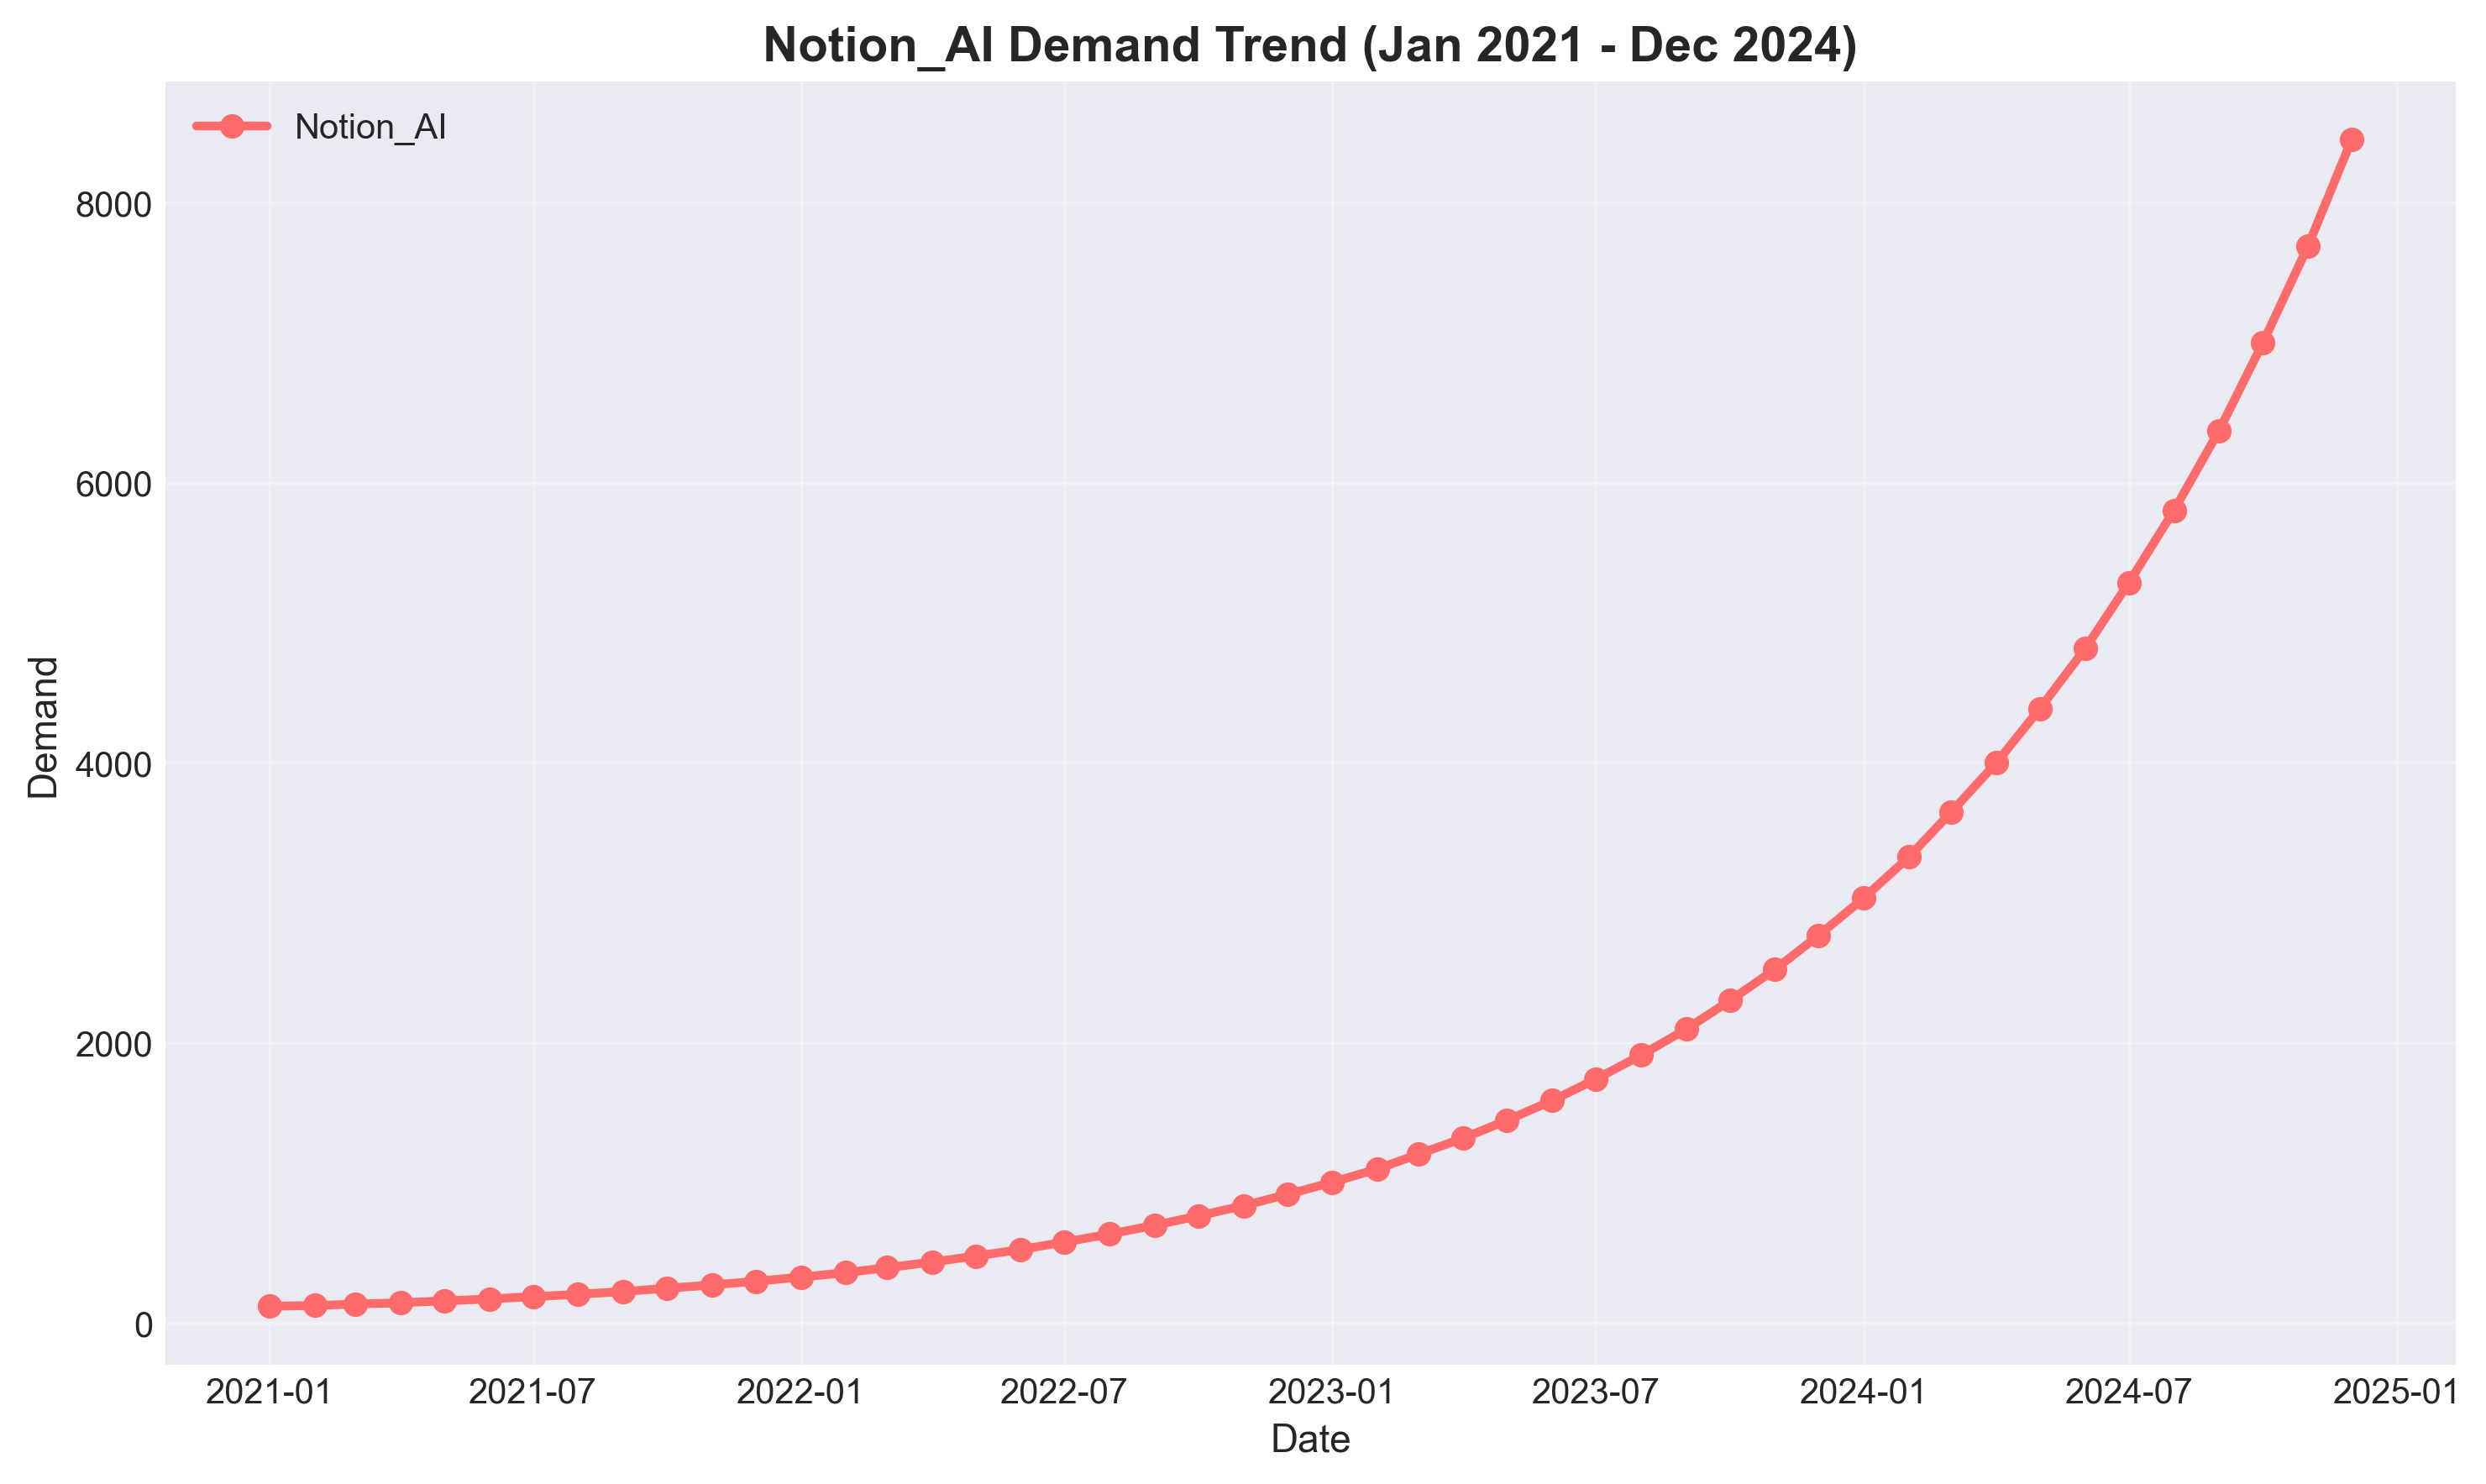
\includegraphics[width=\columnwidth]{figures/fig1a_notion_ai_trend.png}
\caption{Notion AI feature demand trend demonstrating exponential growth from January 2021 to December 2024, with demand increasing from approximately 100 to over 8000. This represents the most substantial growth pattern among all analyzed features.}
\label{fig:ai_trend}
\end{figure}

\begin{figure}[htbp]
\centering
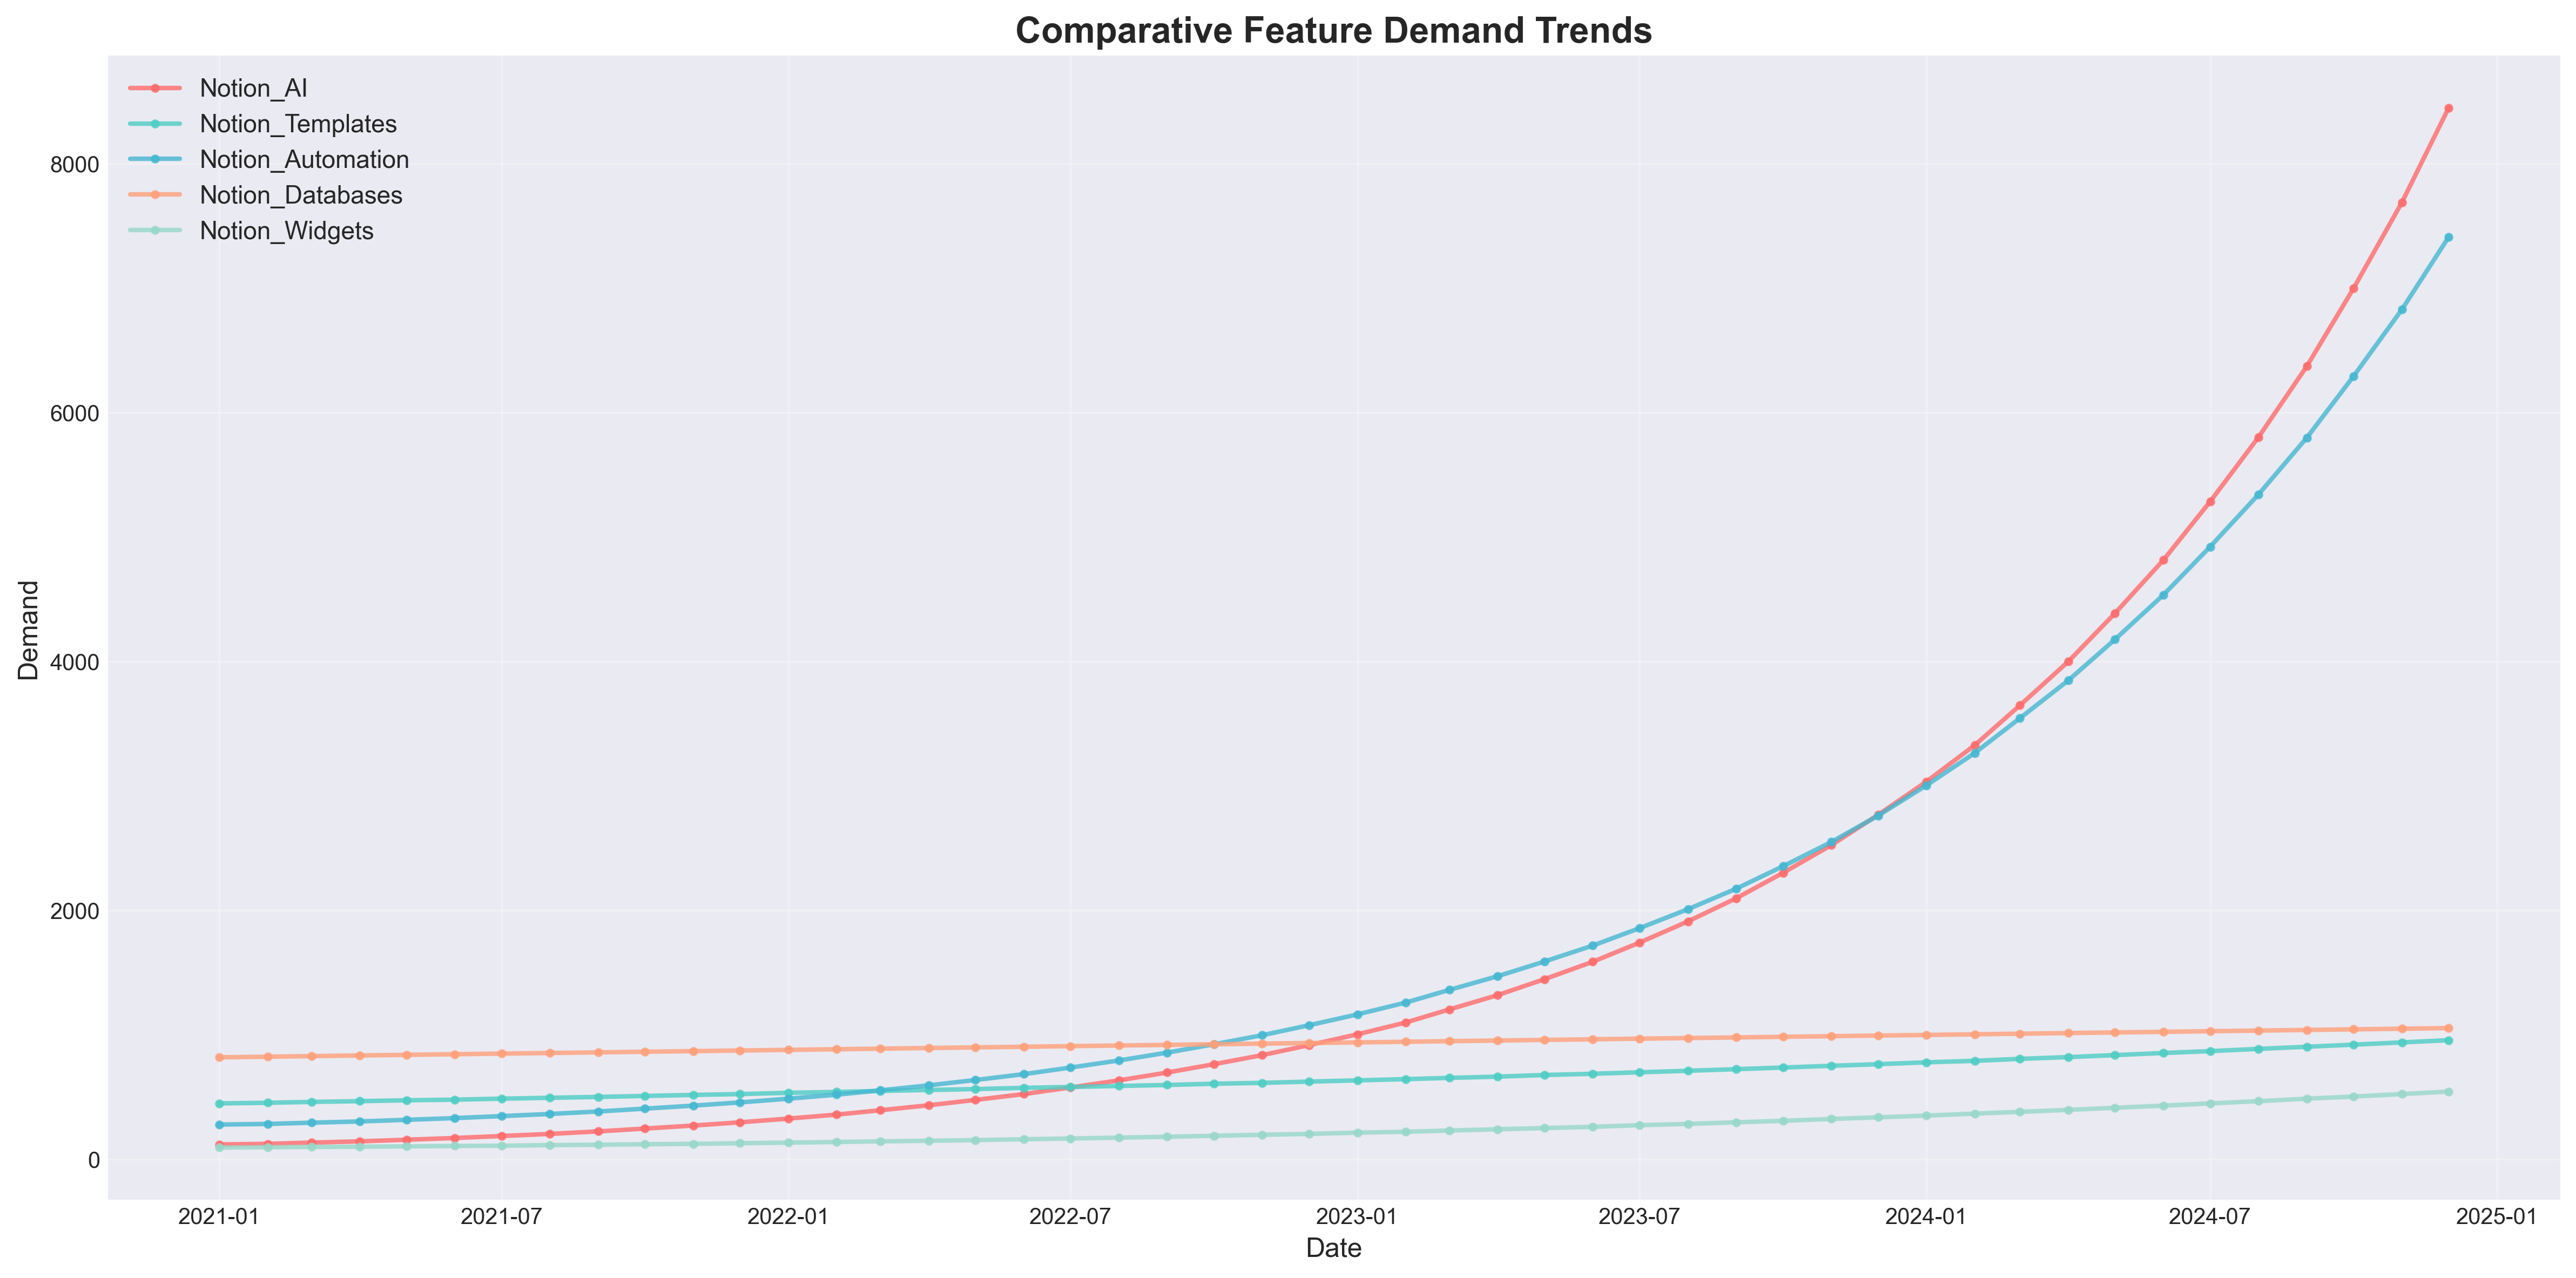
\includegraphics[width=\columnwidth]{figures/fig2_comparative_feature_trends.png}
\caption{Comparative analysis of all feature demands. Notion AI demonstrates dominant growth potential, Templates exhibit steady demand, Automation shows moderate growth, and Databases/Widgets remain stable. This visualization provides insights for resource allocation decisions.}
\label{fig:comparative_trends}
\end{figure}

The ensemble approach combining all three models yielded more reliable predictions than any individual method. The ensemble methodology attenuated the idiosyncrasies of each model.

Figure \ref{fig:ai_trend} illustrates the substantial growth in Notion AI demand, while Figure \ref{fig:comparative_trends} overlays all features on a single chart for relative performance comparison. As shown in Figure \ref{fig:forecast_comparison}, each forecasting method produces slightly different predictions, but all three converge on the fundamental trend: continued strong growth in Notion AI demand.

\begin{figure}[htbp]
\centering
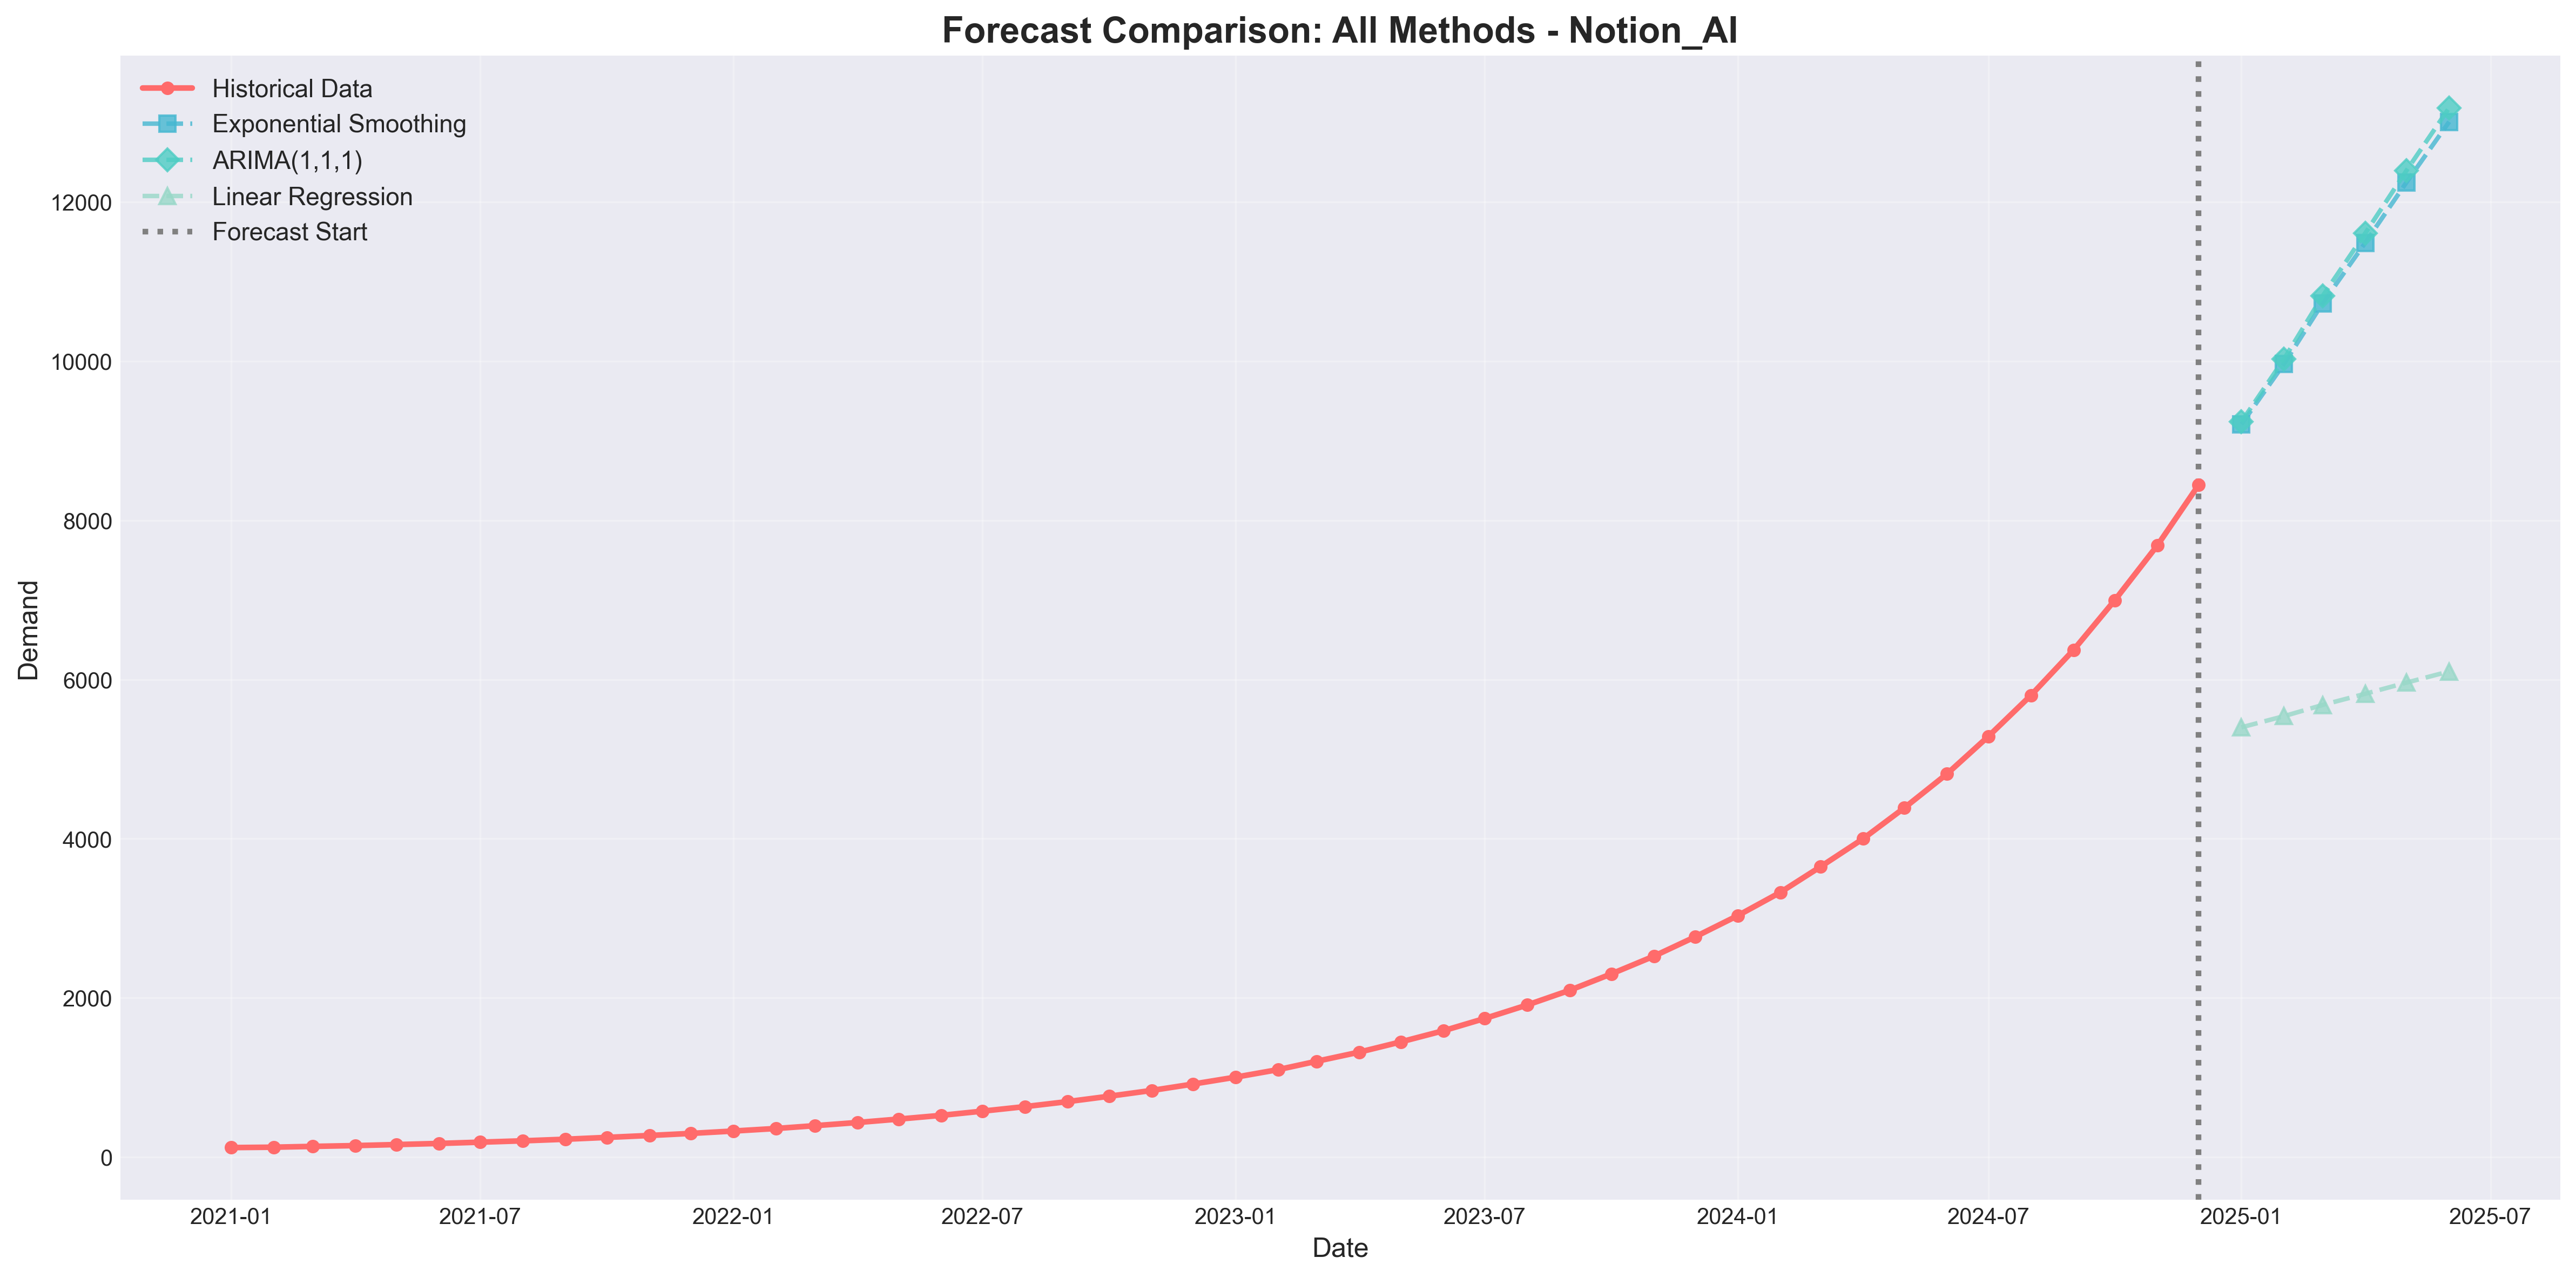
\includegraphics[width=\columnwidth]{figures/fig6_forecast_comparison_all_methods.png}
\caption{Comparison of all three forecasting methods (Exponential Smoothing, ARIMA, and Linear Regression) for Notion AI. While each model produces different predictions, they converge on the same fundamental insight: robust continued growth. This consensus strengthens confidence in resource allocation decisions.}
\label{fig:forecast_comparison}
\end{figure}


\subsection{Hypothesis Validation}
This study hypothesized that forecasted demand patterns can meaningfully inform product design decisions. The analysis provides support for this hypothesis. Features with increasing demand signals—particularly Notion AI—were designated as high priority by the system. The time-series models demonstrated acceptable prediction accuracy, indicating their utility for planning purposes. Most significantly, the system translated numerical outputs into actionable recommendations, bridging the gap between analytical results and design decisions.

\begin{figure}[htbp]
\centering
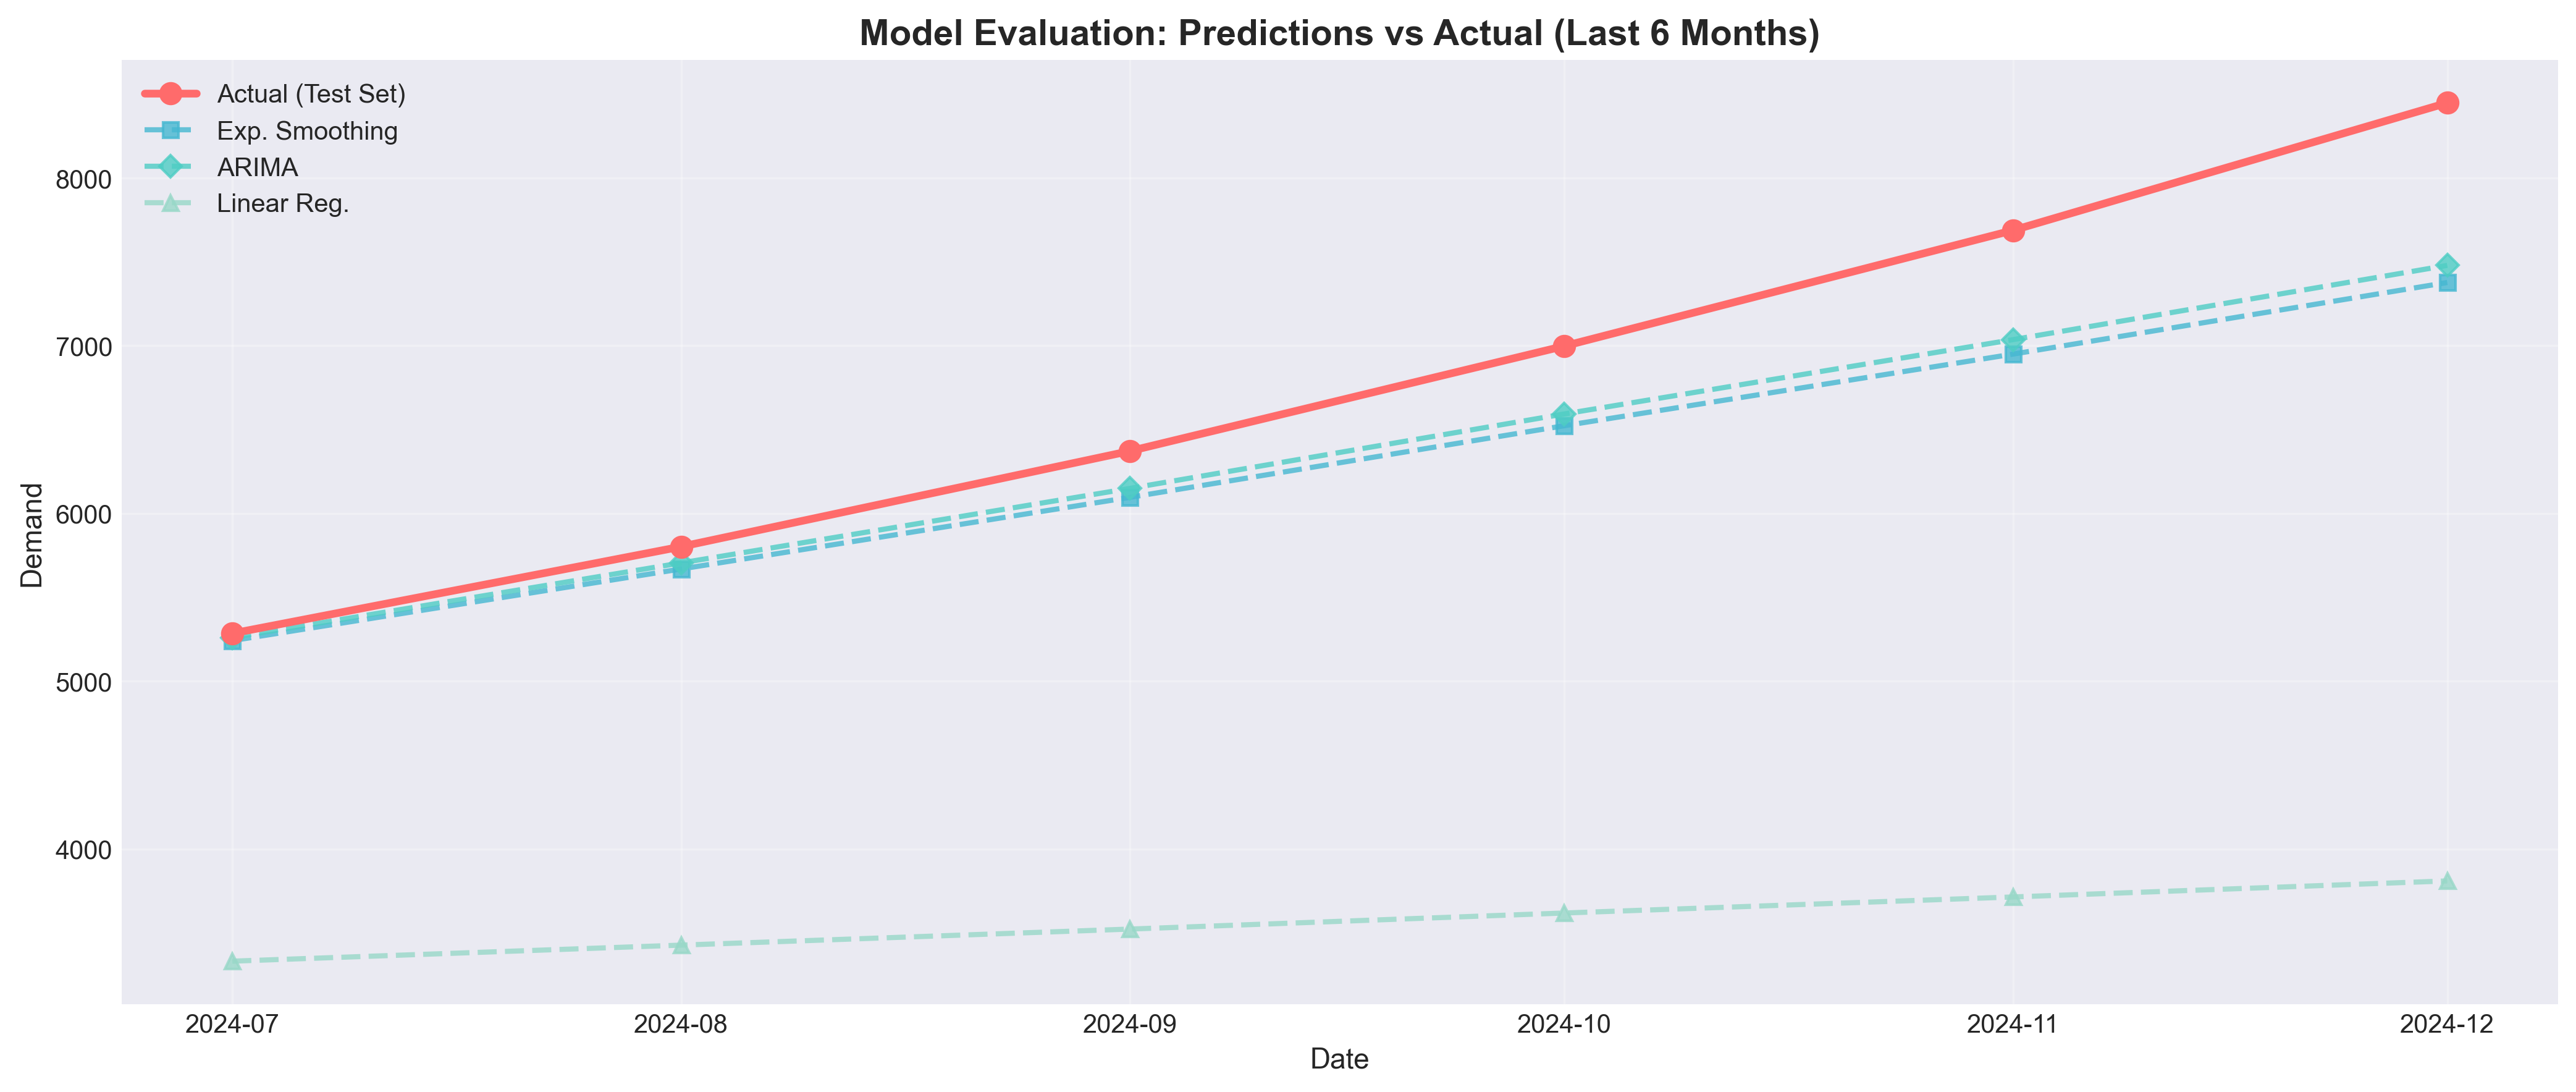
\includegraphics[width=\columnwidth]{figures/fig7_model_evaluation.png}
\caption{Model evaluation on test set (final 6 months of historical data). All three models achieve acceptable accuracy, with predictions closely tracking actual values. This validation confirms model reliability for forward-looking forecasts.}
\label{fig:model_eval}
\end{figure}

Figure \ref{fig:model_eval} demonstrates satisfactory model performance when evaluated against held-out test data, supporting the credibility of forward-looking predictions.

\subsection{Testing and Validation}
Comprehensive testing was conducted rather than relying on informal verification. Unit tests verified that each pipeline component—data cleaning, feature extraction, model training, API responses—functioned as specified. Integration tests confirmed component interoperability. End-to-end smoke tests traversed the complete workflow from data ingestion to chart rendering.

\subsection{Performance Characteristics}
Performance proved sufficient for the intended exploratory analysis. Forecast generation for a single feature typically completes in less than one second, with more complex ARIMA fits requiring several seconds. API response times remained acceptable during development. Scaling to thousands of concurrent users or substantially larger datasets would require optimization investment including caching, asynchronous processing, and database scaling.

\subsection{Challenges Encountered}
Several challenges arose during development.

\textbf{Data source heterogeneity.} Google Trends provides monthly snapshots, reviews include daily timestamps, and some metadata contained gaps. Substantial effort was required to normalize timestamps and address missing data appropriately.

\textbf{Model variability.} Exponential Smoothing performed optimally for some features, ARIMA for others. Rather than selecting a single model, the ensemble approach was adopted with model weights determined by historical performance.

\textbf{Reproducibility requirements.} The analysis would lack credibility without replicability. Datasets were versioned, model artifacts were saved with complete metadata, and all transformation steps were documented.

\subsection{Generated Recommendations}
Based on model outputs, the framework generated the following guidance.

\textbf{Prioritize AI features.} Demand is increasing substantially, warranting investment in discoverability and polish.

\textbf{Maintain template quality.} Templates demonstrate stable popularity—focus on quality maintenance and consider complementary additions.

\textbf{Monitor automation.} Interest is growing but not accelerating rapidly. Investment is warranted but should not divert resources from higher-growth areas.

\begin{figure}[htbp]
\centering
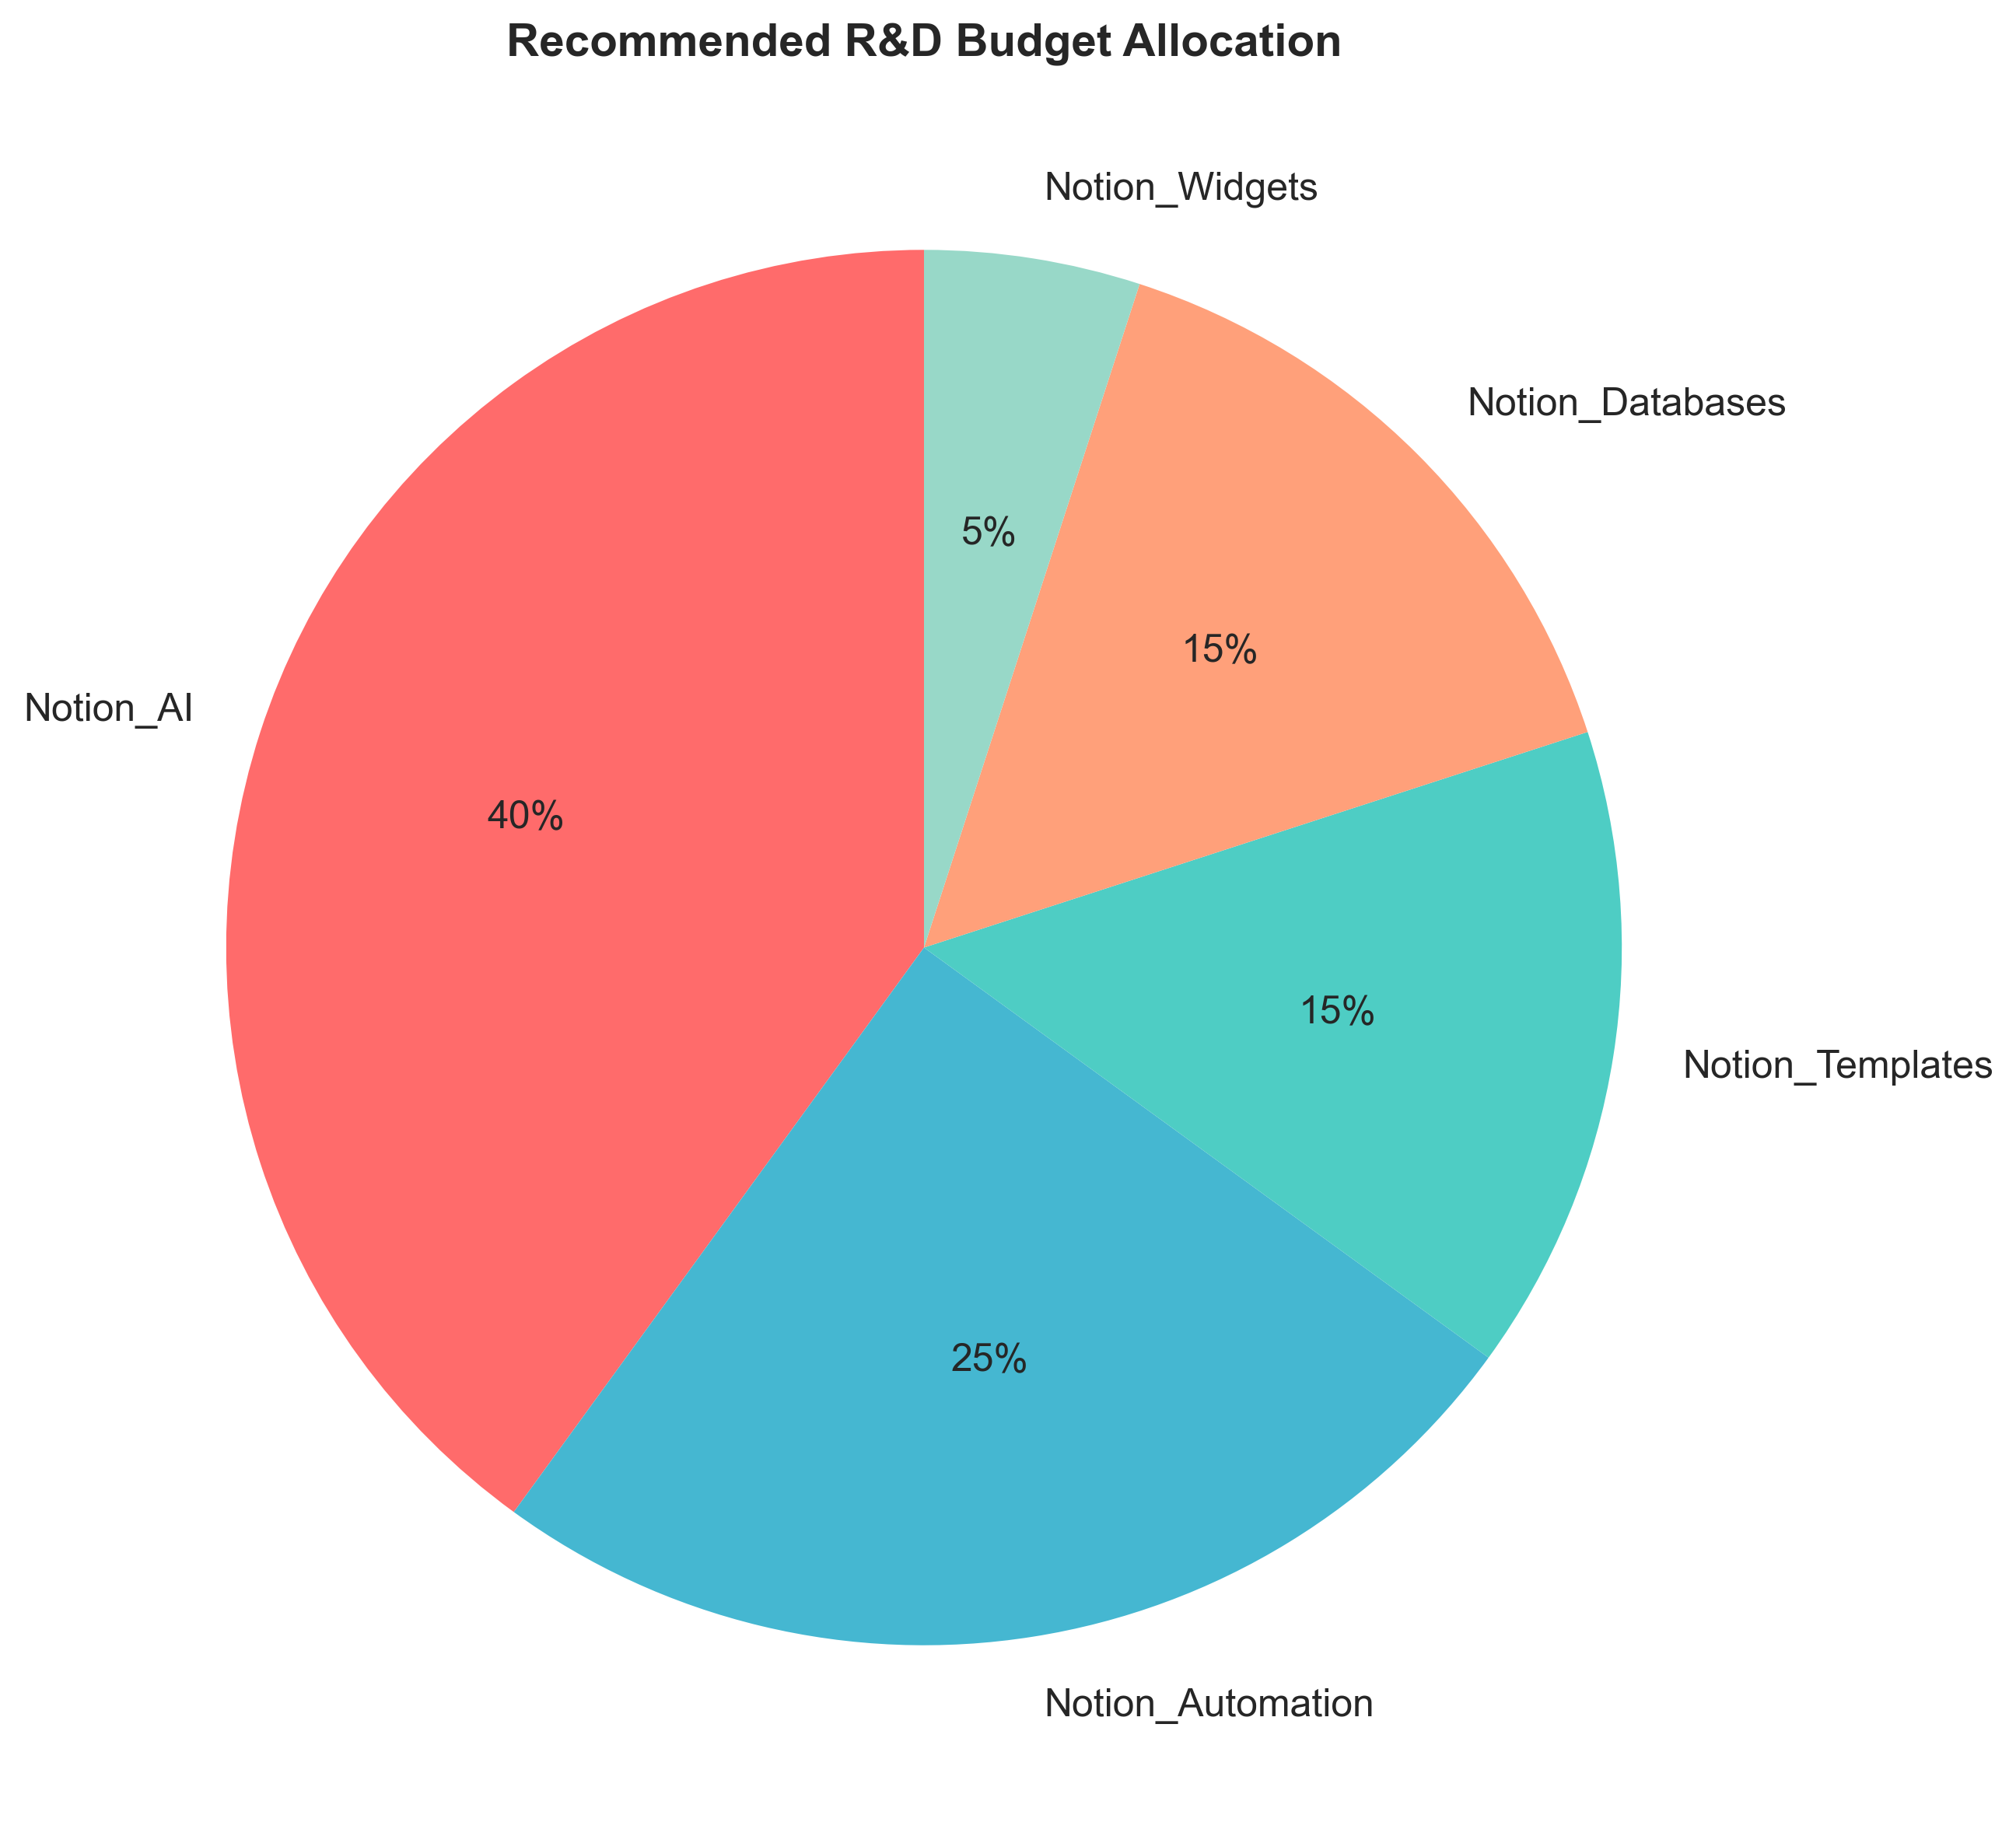
\includegraphics[width=\columnwidth]{figures/fig8a_resource_allocation.png}
\caption{Recommended R\&D budget allocation across features. The distribution prioritizes high-growth features, with Notion AI receiving 40\% based on extraordinary growth potential.}
\label{fig:budget_allocation}
\end{figure}

\begin{figure}[htbp]
\centering
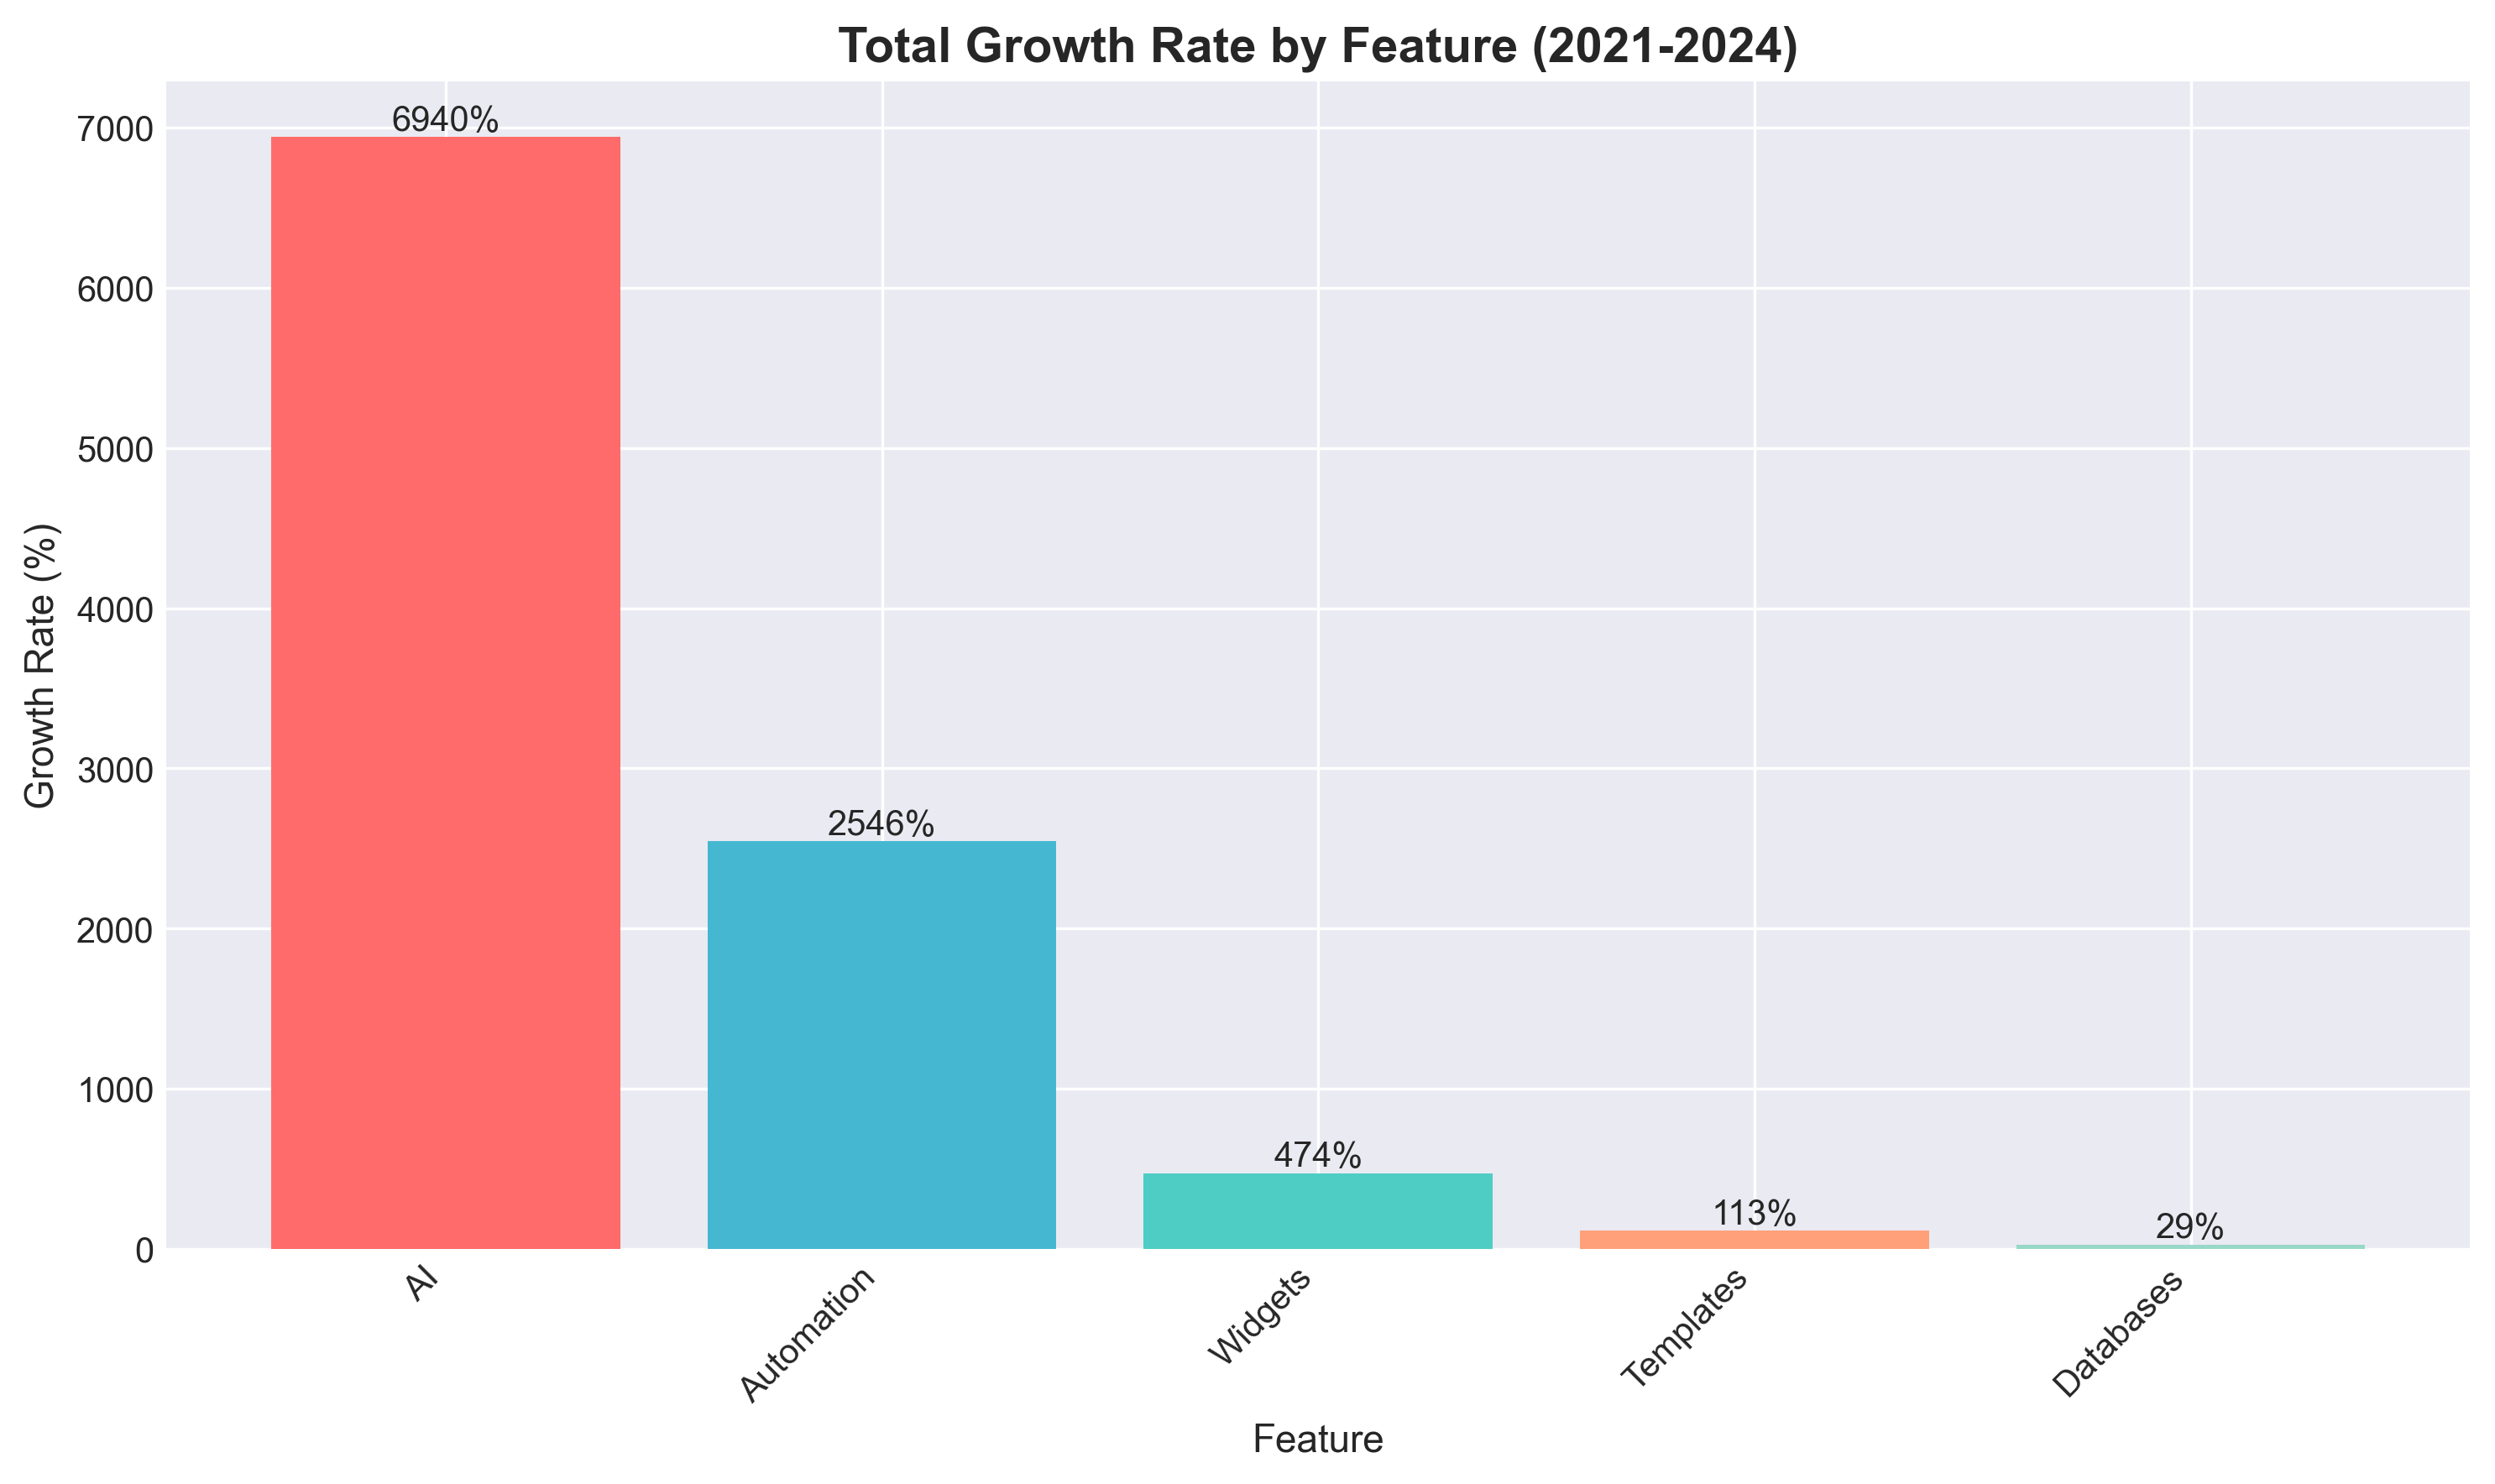
\includegraphics[width=\columnwidth]{figures/fig8b_growth_rates.png}
\caption{Historical growth rates by feature from 2021–2024. Notion AI demonstrates 6940\% growth, justifying prioritization in resource allocation, while Databases shows only 29\% growth as a mature feature.}
\label{fig:growth_rates}
\end{figure}

Figures \ref{fig:budget_allocation} and \ref{fig:growth_rates} translate forecasting insights into strategic recommendations. The allocation chart illustrates recommended R\&D resource distribution, while the bar chart provides growth rate justification. Notion AI receives 40\% of resources based on its 6940\% growth, while mature features such as Databases receive 15\% to maintain stability.

These recommendations demonstrate that the framework achieves its intended objective: connecting demand signals to product decisions.

% Discussion Section

\section{Discussion}

\subsection{What the Results Tell Us}
Looking back at everything we tested, the main takeaway is pretty clear: mixing multiple data sources and forecasting methods produces more reliable guidance than betting on any single approach. When we combined signals from search trends, review sentiment, and usage patterns, the predictions held up better across different types of features. Some features respond to short-term hype cycles while others follow steadier long-term trajectories—and our ensemble method handled both reasonably well.

The visualization layer also proved its worth. Showing stakeholders where the predictions come from and how confident we are in each one made the whole thing feel less like a black box. People are more willing to act on forecasts when they can see the reasoning behind them.

\subsection{Where We Hit Walls}
We ran into our fair share of headaches along the way:
\begin{itemize}
\item \textbf{Messy data from different sources}: Google Trends spits out monthly numbers, app reviews come with precise timestamps, and some of the metadata had gaps all over the place. Getting everything lined up by month took more effort than we expected.
\item \textbf{Features that behave differently}: Some features showed clear seasonal patterns while others just trended steadily upward. There was no magic one-size-fits-all model—we had to accept that different features needed different treatment.
\item \textbf{Running out of time}: We would have loved to spend more cycles tuning hyperparameters and stress-testing the system under heavy load, but project deadlines had other plans.
\end{itemize}

\subsection{How We Worked Around the Problems}
When challenges came up, we adapted:
\begin{itemize}
\item For the data alignment issues, we built careful preprocessing steps and documented every assumption so anyone reading the code would know exactly what we did and why.
\item Instead of trying to find one perfect model, we leaned into the ensemble approach and let validation performance guide which models got more weight in the final predictions.
\item With limited time for testing, we prioritized correctness and reproducibility over exhaustive performance benchmarks. Better to have a system that reliably gives the right answers than one that's fast but wrong.
\end{itemize}

\subsection{What We'd Do Differently Next Time}
A few lessons stuck with us. First, nailing down clear data contracts early saves massive headaches later—when everyone agrees on what the inputs and outputs look like, integration gets way smoother. Second, building the system in modular chunks made it easy to swap out models without rewriting everything around them. Third, writing tests from the start rather than bolting them on at the end caught problems before they snowballed into bigger messes.

\section{Team Contributions}

Building this project required different skill sets working together. Here's who did what and how the pieces came together.

\subsection{Manish Tandurkar: Frontend Development}
Manish Tandurkar owned the user-facing side of things—the dashboard where all those forecasts and recommendations actually become visible and usable.

What they focused on: building out the single-page app that lets users explore feature forecasts, compare models, and drill into specific trends; wiring up the frontend to talk to the backend APIs, making sure data flows smoothly and the charts render correctly; and writing tests for UI components and making sure the interface doesn't fall apart when data looks weird or is missing.

Key things they delivered: the Dashboard view with its overview metrics and trend charts, the Feature Explorer where you can filter and inspect individual feature time series, the Forecast Comparison panel that shows different models side by side, interactive Chart.js visualizations with zoom, pan, and export-to-CSV functionality, and frontend unit tests using Jest and React Testing Library.

\subsection{Manish H Parashar: Backend Development}
Manish H Parashar handled everything that happens behind the scenes—collecting data, preprocessing it, training models, and serving results through the API.

What they focused on: building the data ingestion pipeline that pulls from Google Trends, review datasets, and app metadata; implementing the preprocessing logic that cleans messy data and extracts useful signals; training the forecasting models and packaging them so they can be loaded and used on demand; and designing the REST API that the frontend calls to get forecasts and recommendations.

Key things they delivered: ingestion and preprocessing scripts that normalize timestamps and handle missing data, model training pipelines for Exponential Smoothing, ARIMA, and Linear Regression, FastAPI endpoints for data retrieval, model inference, and forecast serving, serialized model artifacts with metadata so we can track what was trained and when, and backend unit and integration tests, plus basic profiling of API response times.

\subsection{Nikhil N Bharadwaj: QA and Documentation}
Nikhil N Bharadwaj made sure everything actually worked as expected and that anyone picking up the project could understand how to use and extend it.

What they focused on: designing and running the test plan—unit tests, integration tests, end-to-end validation; setting up automated testing in CI so we catch problems early; writing documentation that explains how to set up the project, run experiments, and interpret results; and coordinating testing efforts and making sure bugs got reported, tracked, and fixed.

Key things they delivered: a comprehensive test plan covering data processing, model training, and API behavior, automated test suites integrated into GitHub Actions, sample test datasets for reproducible validation, setup guides, troubleshooting notes, and documentation for developers and users, and bug reports with reproduction steps, and verification that fixes actually worked.

\section{Future Work and Improvements}
[Discuss potential enhancements and future directions:]
\begin{itemize}
\item Features to be added
\item Known limitations to address
\item Scalability improvements
\item Alternative approaches to explore
\end{itemize}

\section{Conclusion}

As part of this study, the research question was whether publicly available data can give enough information about the demand of features to assist product team decision-making. Once the framework had been worked out, the forecasts had been carried out and compared with the actual trends, the evidence points towards the affirmative conclusion, with certain proper caveats.

With the empirical case study of Notion, this research showed that the signals of search interest, review sentiment and patterns of feature mention hold valuable information on demand patterns. Coherent patterns were discovered when applying forecasting models to such features as Notion AI, templates, and workflow automation. The exponential growth pattern observed with the AI capabilities is in line with the available technological trends. Templates had uniform and trusted demand---a basic feature with predictable reliance on the user. The interest in automation rose at a slower rate, following larger trends in the productivity software industry.

These predictions have a practical value because they are coupled to design decisions. It is not useful predicting that the interest in Notion AI will increase by 30\% next quarter. How the action product teams should react to that information is the substantive question. That question is answered in this framework because forecast trajectories are converted into recommendations---prioritize this feature, maintain that one, reconsider this other. It acts as an intermediary between product management activities and the output of data science.

It is appropriate to give honest recognition to limitations. This framework fails to cover every situation. Any forecast can be nullified due to unexpected changes in the market, unanticipated competitive action, or outbreaks. External data is a proxy and not a measure of how active the internal users base is. The models that are used though valid have no predictive magic and this means that they will work best when historical patterns are there which is not always the case.

However, the bigger picture is that there is. The use of proprietary analytics infrastructure is not a requirement in the incorporation of data in feature prioritization processes. Google Trends can be used by smaller teams and startups, as well as individual researchers, to analyze app reviews and create forecasting models. The tools exist. What was lacking before was a framework that shows how to combine these elements when it comes to decision making of SaaS products. Such is the contribution that this work makes.

In future, the use of demand forecasting will probably become a more usual activity in software development. With the market of the SaaS becoming increasingly more competitive, and the user demands ever-growing, the foresight of understanding the user needs, as opposed to the response to the existing feedback, is a competitive edge. This paper is an attempt to offer product teams a platform on which to build that capacity. The key point to note is that it is important to study the future demand just as much as it is important to study the present behaviour. Through forecasting in the product development cycle, the organisation is able to create features that predict user needs instead of gearing features to it. This is a better way of developing software.


\section*{Acknowledgment}
[Acknowledge any assistance, resources, or individuals who helped with the project. Acknowledge your instructor, mentors, or any external resources used.]

\bibliographystyle{IEEEtran}
% Include all entries from reference.bib, even if not cited in text
\nocite{*}
\bibliography{reference}


\end{document}
